\chapter{Planning and Methodology}

Before getting into details on the system design and development, this section will explain the selection of the engineering methodology and the way it is applied in this project.

\section{Methodology}

A Kanban board is used to manage project tasks using an incremental method, organizing them into \textit{To Do}, \textit{In Progress} (further divided into \textit{Working} and \textit{Waiting}) and \textit{Done} columns. This structure avoids bottlenecks and facilitates visibility of the status of each activity. Moreover, by focusing on reducing waste (overproduction, unnecessary movements, defects, overprocessing and waiting), it minimizes downtime and optimizes workflow \cite{ref43}. In addition, an initial project planning will be performed, progress will be monitored, deviations will be adjusted and regular meetings will be held with the director.

Also, prototyping is used for the assembly and functionality development of hardware modules. It helps to rapidly develop and test new ideas and designs before final production. In hardware design, prototyping is essential to validate concepts, explore design alternatives and detect problems early on. It is an iterative process in which multiple versions of the design are created, tested and refined; allowing adjustments and improvements based on continuous testing and feedback \cite{ref44}. In this project, every module that is intended to be added to the project is tested in an isolated way, before adding it to the complete system, to check whether it is able to perform all its functionalities.

\subsection{Hardware Prototyping Planning}

The adoption of an iterative development cycle at the hardware layer is intended to validate physical components (Arduino Uno, MFRC522 and ESP32) independently, allowing for quick adjustments to wiring, SPI/UART configurations and test codes before advancing to the next phase.

In order to adopt this methodology, the following iterations were defined:

\begin{itemize}
	\item Iteration 1: Basic NFC communication.
	\item Iteration 2: Providing basic Wi-Fi connectivity.
	\item Iteration 3: Mutual authentication and writing in NFC card Memory.
	\item Iteration 4: Reading NFC Card memory and Loading Cryptographic Keys.
	\item Iteration 5: NACU Subsystem Full Integration.
	\item Iteration 6: Magnetic lock Management for Physical Access Control.
\end{itemize}

\subsection{Incremental Planning for Backend \& HSM}

To adapt incremental development to the Django server and HSM logic, five delivery cycles were defined with several deliverables attached to each one of them:

\begin{itemize}
	\item Iteration 1: Basic Structure and Authentication.
	\item Iteration 2: Key Derivation System.
	\item Iteration 3: Transport encryption (HTTPS/TLS).
	\item Iteration 4: Real Time Access Control Mail Alert System.
	\item Iteration 5: Role-Based Access Control.
\end{itemize}

\subsection{Deliverables}

\begin{table}[H]
	\small
	\begin{tabular}{|c|p{5cm}|c|p{3.5cm}|}
		\hline
		\textbf{Code} & \textbf{Description} & \textbf{Iteration} & \textbf{Validation} \\ \hline
		1  & Setup Django project with login and admin default panel. & 1 & \multirow{4}{*}{\parbox{3.5cm}{Persistence of UIDs and verification of time slots.}} \\ \cline{1-3}
		2  & Persistence of UIDs and verification of time slots. & 1 & \\ \cline{1-3}
		3  & Create a view that allows visualization of access attempts. & 1 & \\ \cline{1-3}
		4  & Create data models for users and schedules. & 1 & \\ \hline
		5  & Create endpoints for submitting and authenticating users. & 1 & \multirow{3}{*}{\parbox{3.5cm}{JSON response with 32 hex key characters.}} \\ \cline{1-3}
		6  & Endpoint for HMAC-SHA256 key derivation. JSON response with 32 hex key characters. & 2 & \\ \cline{1-3}
		7  & Software implementation of Hardware Security Module. & 2 & \\ \hline
		8  & File I/O management and error control. & 2 & \multirow{2}{*}{\parbox{3.5cm}{Secure connection https:// encrypted in development.}} \\ \cline{1-3}
		9  & Evolution to HTTPS. Secure connection https:// encrypted in development. & 3 & \\ \hline
		10 & Wi-Fi module adaptation for working with HTTPS. & 3 & \multirow{2}{*}{\parbox{3.5cm}{Receiving emails after unauthorized access.}} \\ \cline{1-3}
		11 & SMTP configuration. Receiving emails after unauthorized access. & 4 & \\ \hline
		12 & Code functionality to send mail. & 4 & \multirow{2}{*}{\parbox{3.5cm}{Prototype.}} \\ \cline{1-3}
		13 & Reader detection. Prototype. & 5 & \\ \hline
		14 & Creation of Role model. & 5 & \\ \hline
	\end{tabular}
	\caption{Incremental Methodology list of Deliverables for the different iterations of the incremental ACMS development}
	\label{tab:deliverables}
\end{table}


\section{Project Planning, Monitoring and Controlling}

This section describes the processes and tools used to ensure that prototype development met its objectives in terms of scope, schedule and budget. Emphasis is placed on continuous planning, monitoring and control of tasks to ensure on-time delivery, traceability of changes and compliance with quality criteria throughout the project life cycle.

\subsection{Monitoring Tools}

\paragraph{Kanban:} For both iterative and incremental prototyping development, a Kanban board was used with \textit{To Do}, \textit{In Progress}, \textit{Test} and \textit{Done} columns. Each board describes a specific task (e.g: UID read, EV2 authentication, NDEF write, endpoint creation).

\begin{figure}[H]
	\centering
	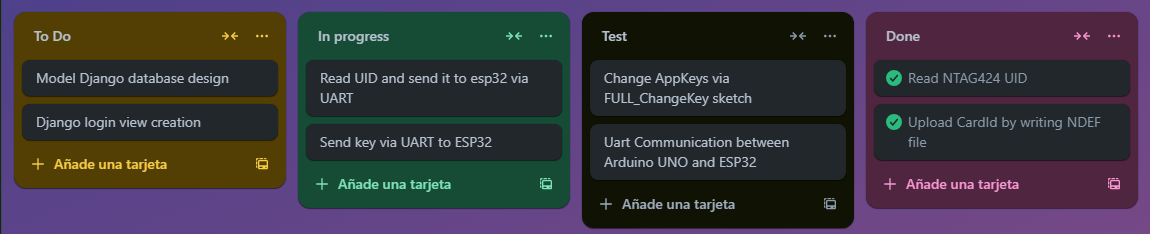
\includegraphics[width=0.7\textwidth]{imaxes/kanban.png} % Insert your image path here
	\caption{Kanban Board at Early Stages of the Project}
	\label{fig:kanban}
\end{figure}

\paragraph{Version control on GitHub:} During the development of both the Arduino/ESP32 scripts and the Django/HSM backend, each progress is recorded through “commits” in a single repository on GitHub. In this way, a detailed history of changes to all project components is maintained, facilitating collaboration, version tracking and retrieval of previous states when necessary \cite{ref52, ref53}.

\subsection{Gantt Chart and Timing Resources}

A Gantt chart was developed in Excel to estimate the “goals” of each iteration and their approximate duration (total 300 hours).

Main phases:
\begin{itemize}
	\item State of the Art research.
	\item Write project draft.
	\item Researching on Arduino Uno, MFRC522 and ESP32 technology.
	\item Researching on NTAG424 technology.
	\item System design and analysis.
	\item Iterative hardware prototyping.
	\item Testing MFRC522-NTAG424 functionalities.
	\item Incremental backend Access Control Management Server implementation.
	\item Full system integration and testing.
	\item Degree thesis.
\end{itemize}


\begin{figure}[H]
	\centering
	\includegraphics[width=20cm]{imaxes/gantt1.png} % Insert your image path here
	\caption{Gantt Diagram representing all the phases of the project and the time in weeks that was spent on each one, along with its deviation from the original duration}
	\label{fig:gantt}
\end{figure}

\subsection{E2E Validation and Testing}

After each hardware iteration, manual tests (NFC read/write) were executed.

On the hardware, simple tests were performed on each iteration to ensure proper communication worked.

On the backend, functional tests were performed using petitions in the browser to REST endpoints and mail tests (SMTP).

Finally, several tests were performed on the final system to ensure its capacity to consequently perform the tasks necessary for the data flow to function.

\subsection{Materials and Cost Estimate}

This section details the material resources and their associated cost for the development, deployment and testing of the prototype. All prices are approximate, obtained from online stores as of this writing.

\paragraph{Prototyping and access control hardware:}

\begin{itemize}
	\item Arduino Uno: 22 €.
	\item MFRC522 module (NFC reader): 8 €.
	\item ESP32 module: 10 €.
	\item Standard protoboard (830 points): 5 €.
	\item Basic wiring (male-male jumpers, USB, power supply): 6 €.
	\item Dollatek DC 0-5 V relay module: 7 €.
	\item Electric magnetic lock LIBO 12 V, 180 kg: 28.59 €.
	\item Power adapter 12 V 1.5 A: 8 €.
	\item DC 12 V male-female adapter: 4 €.
\end{itemize}

Total access control hardware: 98.59 €.

\paragraph{Development and testing infrastructure:}

\begin{itemize}
	\item Personal Computer (Django server development and testing): Cost valued at 1,200 € with estimated useful life of 4 years → 0.82 €/day.
	\item Browsers for testing (Opera and Microsoft Edge): no additional cost (free software).
	\item Total software and PC infrastructure (180 days estimated): 147.60 €.
\end{itemize}

\paragraph{Human resources:}

For this project, the working personnel are:

\begin{itemize}
	\item A responsible for system design and implementation, whose cost was estimated using the calculator provided by the UDC \cite{ref60}, which resulted in a total cost of 28,574.31 €.
	\item A project manager role, represented by the tutor whose work was estimated to last 45 hours at a cost of 100 € per hour, resulting in 4,500 €.
\end{itemize}

Total human resources cost (320 hours estimated): 8,151.5 €.

\begin{table}[H]
	\centering
	\begin{tabular}{|l|r|}
		\hline
		\textbf{Resource} & \textbf{Cost} \\ \hline
		Hardware & 98.59 € \\ \hline
		Software & 147.60 € \\ \hline
		Human & 8,151.5 € \\ \hline
		\textbf{Total} & \textbf{8,397.69 €} \\ \hline
	\end{tabular}
	\caption{Hardware, Software and Human costs of the project}
	\label{tab:costs}
\end{table}
